\section{Modifying and applying RISE (single pixel)}
\nblink{brats/06\_rise.ipynb}

The approach how to apply RISE on a segmentation task the same as with Grad-CAM in the last chapter. Pixels in the output of a segmentation model are equivalent to classes of a classification model.
As a first version, we only analyze a single pixel. We chose the first pixel in the tumor ground truth segment by iterating over the segment linearly until the first active pixel is found.

In the standard implementation, RISE analyzes every class that is returned by the network. Our segmentation model returns $ image_height * image_width $ count classes. This are too many
and the algorithm crashes with an out of memory error. We modified the code to only analyze the output neuron for our selected pixel.

\subsection{Results}

\begin{figure}[H]
\centering
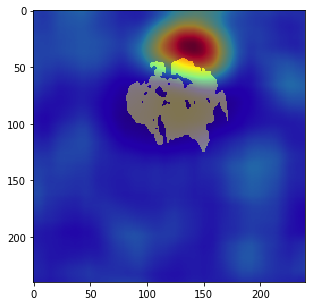
\includegraphics[width=8cm]{chapters/04_segmentation/images/rise_single_pixel.png}
\caption{RISE Saliency map analyzing the topmost pixel in the scan, overlaid on the binarized network output}
\label{rise_single_pixel_result}
\end{figure}

Figure \ref{rise_single_pixel_result} shows the output 

\subsection{Discussion}
The produced output in Figure \ref{rise_single_pixel_result} looks correct, the color blob is at the expected position. It clearly shows that the neural network looks at the correct location to generate the segmentation.
Apart from this basic correctness verification, no further insight is provided by the saliency map, because the resolution generated by RISE is too low.

\subsection{Conclusion}
The generated output is low resolution but still helpful, we therefore decided to build a version of RISE which works on all pixels of the segmentation.

\section{Modifying and applying RISE (multi pixel)}
\nblink{brats/17\_rise\_multipixel.ipynb}

As written in the previous section, RISE crashes when running on all the pixels in the output of the model. We already modified the algorithm to only work on a single pixel. For this multi pixel variant, we extended the algorithm to work on all pixels in the segmentation ground truth. We batched the pixels into groups of 1000 pixels each, because depending on the size of the output segment the algorithm still crashed.

With this changed algorithm, we generate a saliency map like Figure \ref{rise_single_pixel_result} for every single pixel in the output segment.

To have a single saliency map for all pixels, we use the max and mean functions of numpy on the whole set of saliency maps.

\subsection{Results}

\begin{figure}[H]
    \centering
    \begin{subfigure}[t]{.4\textwidth}
        \centering
        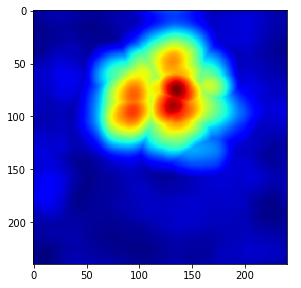
\includegraphics[width=\linewidth]{chapters/04_segmentation/images/rise_multipixel_max_1-0.png}
        \caption{Saliency map created by the max function}
    \end{subfigure}\hspace{1cm}%
    \begin{subfigure}[t]{.4\textwidth}
        \centering
        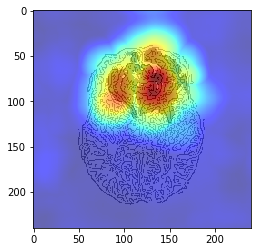
\includegraphics[width=\linewidth]{chapters/04_segmentation/images/rise_multipixel_max_1-1.png}
        \caption{Saliency map created by the max function, overlaid on the binarized network output}
    \end{subfigure}
    \caption{Single saliency map over all output pixels generated by applying the max function on the set of all saliency maps.}
    \label{rise_multipixel_max}
\end{figure}

\begin{figure}[H]
    \centering
    \begin{subfigure}[t]{.4\textwidth}
        \centering
        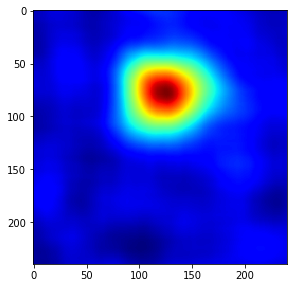
\includegraphics[width=\linewidth]{chapters/04_segmentation/images/rise_multipixel_mean_2-0.png}
        \caption{Saliency map created by the mean function}
    \end{subfigure}\hspace{1cm}%
    \begin{subfigure}[t]{.4\textwidth}
        \centering
        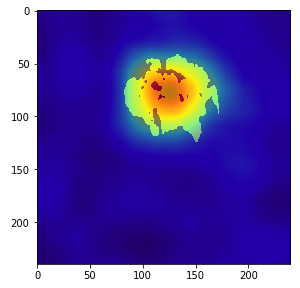
\includegraphics[width=\linewidth]{chapters/04_segmentation/images/rise_multipixel_mean_2-1.png}
        \caption{Saliency map created by the mean function, overlaid on the binarized network output}
    \end{subfigure}
    \caption{Single saliency map over all output pixels generated by applying the mean function on the set of all saliency maps.}
    \label{rise_multipixel_mean}
\end{figure}

\subsection{Discussion}
Figure \ref{rise_multipixel_max} shows a single saliency map matching quite well with the binarized network output. The resolution of the generated saliency map
is quite low, and not many insights can be gathered from it.

The Figure \ref{rise_multipixel_mean} which was generated with the mean function also shows a heat map matching the binarized network output, although with much less detail than the map generated with the max function.

\subsection{Conclusion}
The modified RISE method provides useful insight into the correctness of the model. It clearly marks the important regions the neural network uses to generate the segmentation output. However, the generated saliency map is of low resolution and does only provide a coarse look into the inner workins of the model. Increasing the quantity of used masks by RISE is possible, but generating a single RISE output already takes around 30 seconds on a high-end consumer GPU with 6000 masks. To generate a higher resolution saliency map, many more masks would be required.
